%-------------------------------------------------
% FileName: chap-4.tex
% Description: 第4章 系统总体设计
%-------------------------------------------------

\chapter{系统总体设计}

\section{系统架构设计}

\subsection{前后端分离架构设计}

该系统是前后端分离结构的。前端项目主要实现页面展示、路由跳转、表单校验以及接口调用，后端项目主要是做登录认证、业务规则的判断以及对数据库的操作。两端之间通过 HTTP 接口传递 JSON 数据，前端统一以 /api 作为接口前缀，并在 Axios 请求拦截器中携带 JWT；后端使用 Spring Boot 提供接口，控制器根据认证、场地、订单、器材、用户等业务进行划分，再由 service 层处理具体逻辑，mapper 层完成数据库访问。

这种架构更适合本课题，系统既存在用户端又存在管理端，但是它们共享同一批后端数据。用户端的场地列表调用 /api/venues 查询可预约场地，管理端通过场地维护接口修改同一张场地表；用户提交订单后，个人订单页和后台订单页都能看到相应的记录，但是查询范围不同。前后端分离之后，页面布局及交互修改不会影响后端业务规则，后端接口也可以在不改变页面结构的情况下补充校验逻辑。

\begin{figure}[htbp]
\centering
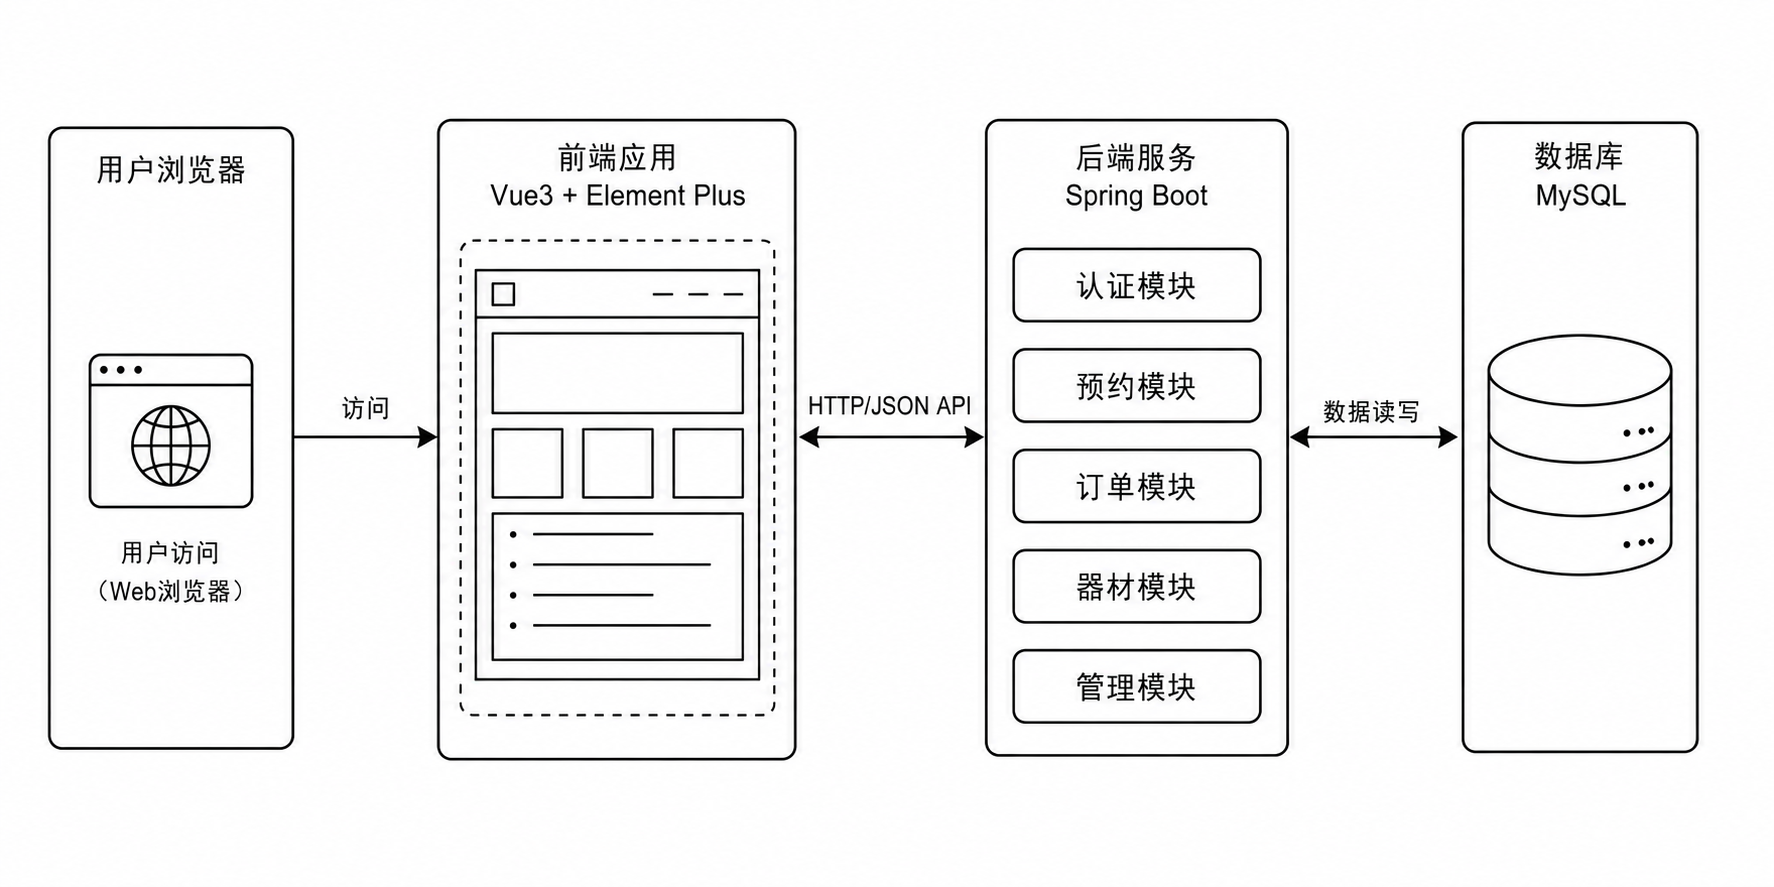
\includegraphics[width=0.82\textwidth]{img/fig4-1.png}
\caption{前后端分离架构图}
\label{fig:architecture-placeholder}
\end{figure}

\subsection{系统模块划分设计}

按照使用角色和业务边界，可以将系统分为用户端模块、管理端模块和公共支撑模块。用户端模块面向普通师生，包括注册登录、场地查询、预约下单、我的订单、器材租借、租借记录查询等。该模块重视操作路径短，用户选择场地之后只需要确定日期、开始时间和结束时间，即可生成待支付订单。

管理端模块面向管理员，有后台首页、场地管理、订单管理、器材管理、用户管理。本模块的重点并不是界面的数量，而是维护数据的一致性，场地上下架会影响用户端是否展示，器材数量修改要考虑已经借出的数量，用户角色调整会改变后台的访问权限。公共支撑模块是第一、二类功能的延伸，包含 JWT 鉴权、管理员权限判断、统一返回结果封装、全局异常处理以及分页查询等。将这些支撑能力从各个业务接口中抽取出来，可以减少各业务接口中的重复代码，也可以使得前端对于成功和失败的响应使用较为一致的处理方式。

\begin{figure}[htbp]
\centering
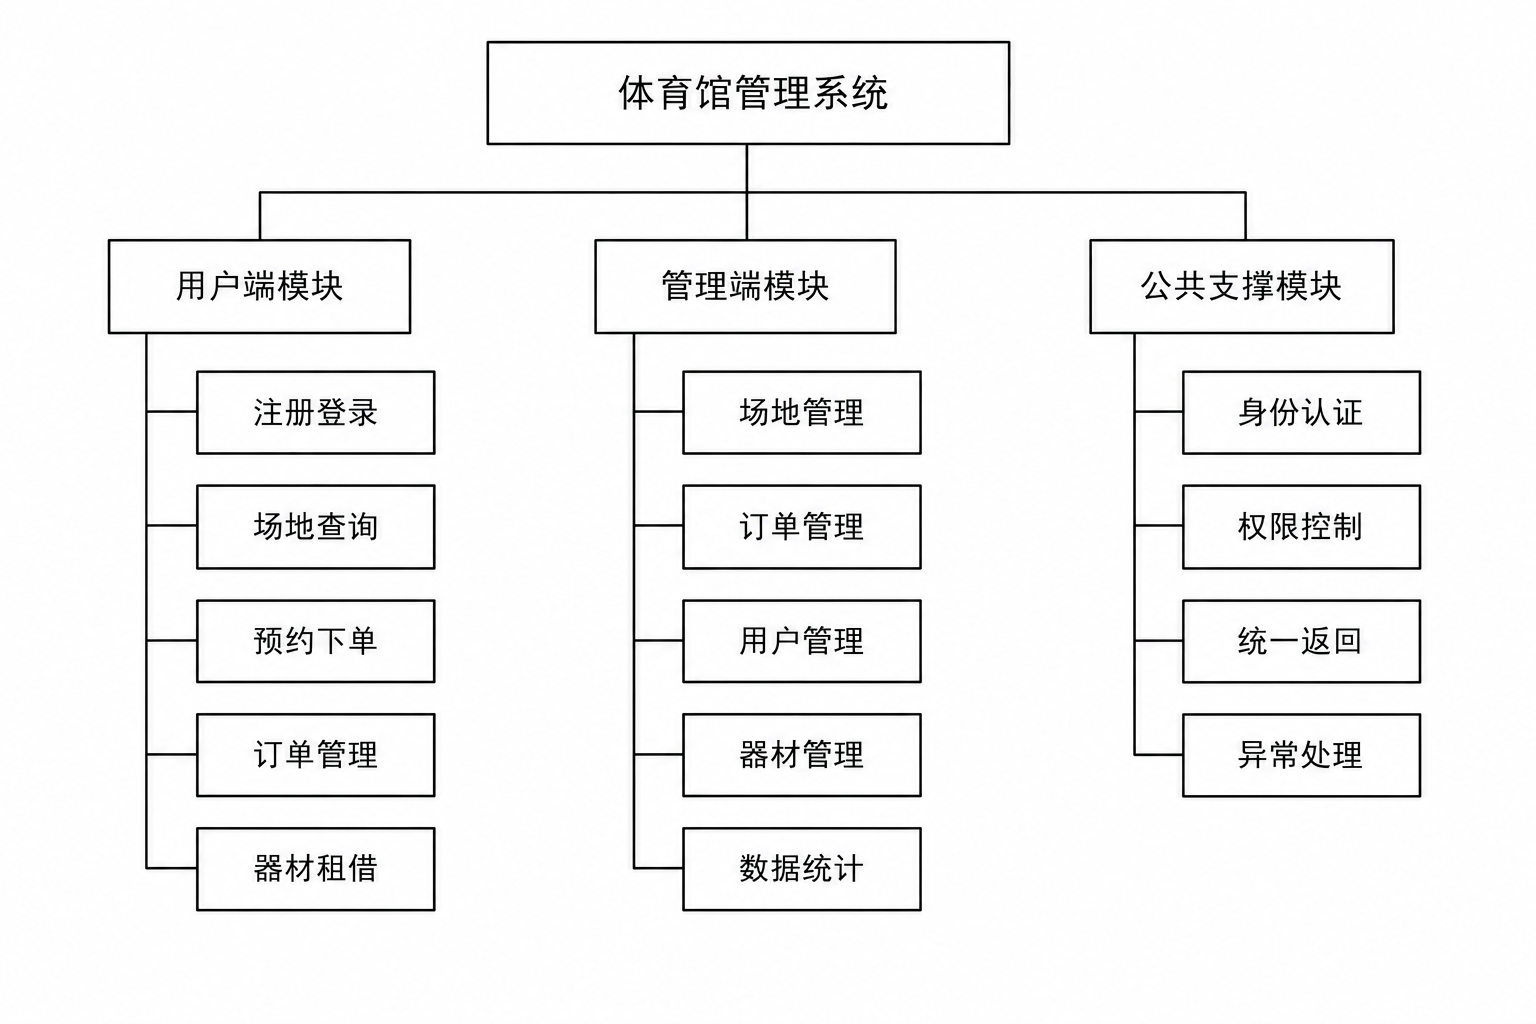
\includegraphics[width=0.82\textwidth]{img/fig4-2.png}
\caption{系统功能模块图}
\label{fig:module-placeholder}
\end{figure}

\subsection{核心业务流程设计}

系统中两条主线需要单独画出流程。第一条是场地预约：用户登录后进入场地列表，根据题目给出的条件选择一个合适的场地、日期和时段后提交预约申请，系统后端校验冲突并生成订单，订单进入“待支付”状态等用户后续支付或取消。第二条是器材租借：用户在器材列表里查看库存、提交租借申请、后端扣减可借数量并生成租借记录，当管理员在后台进行归还操作的时候再把数量加上去。两条主线提前梳理好之后，就可以在后面的设计与关系图中更好地呈现出来。

\begin{figure}[htbp]
\centering
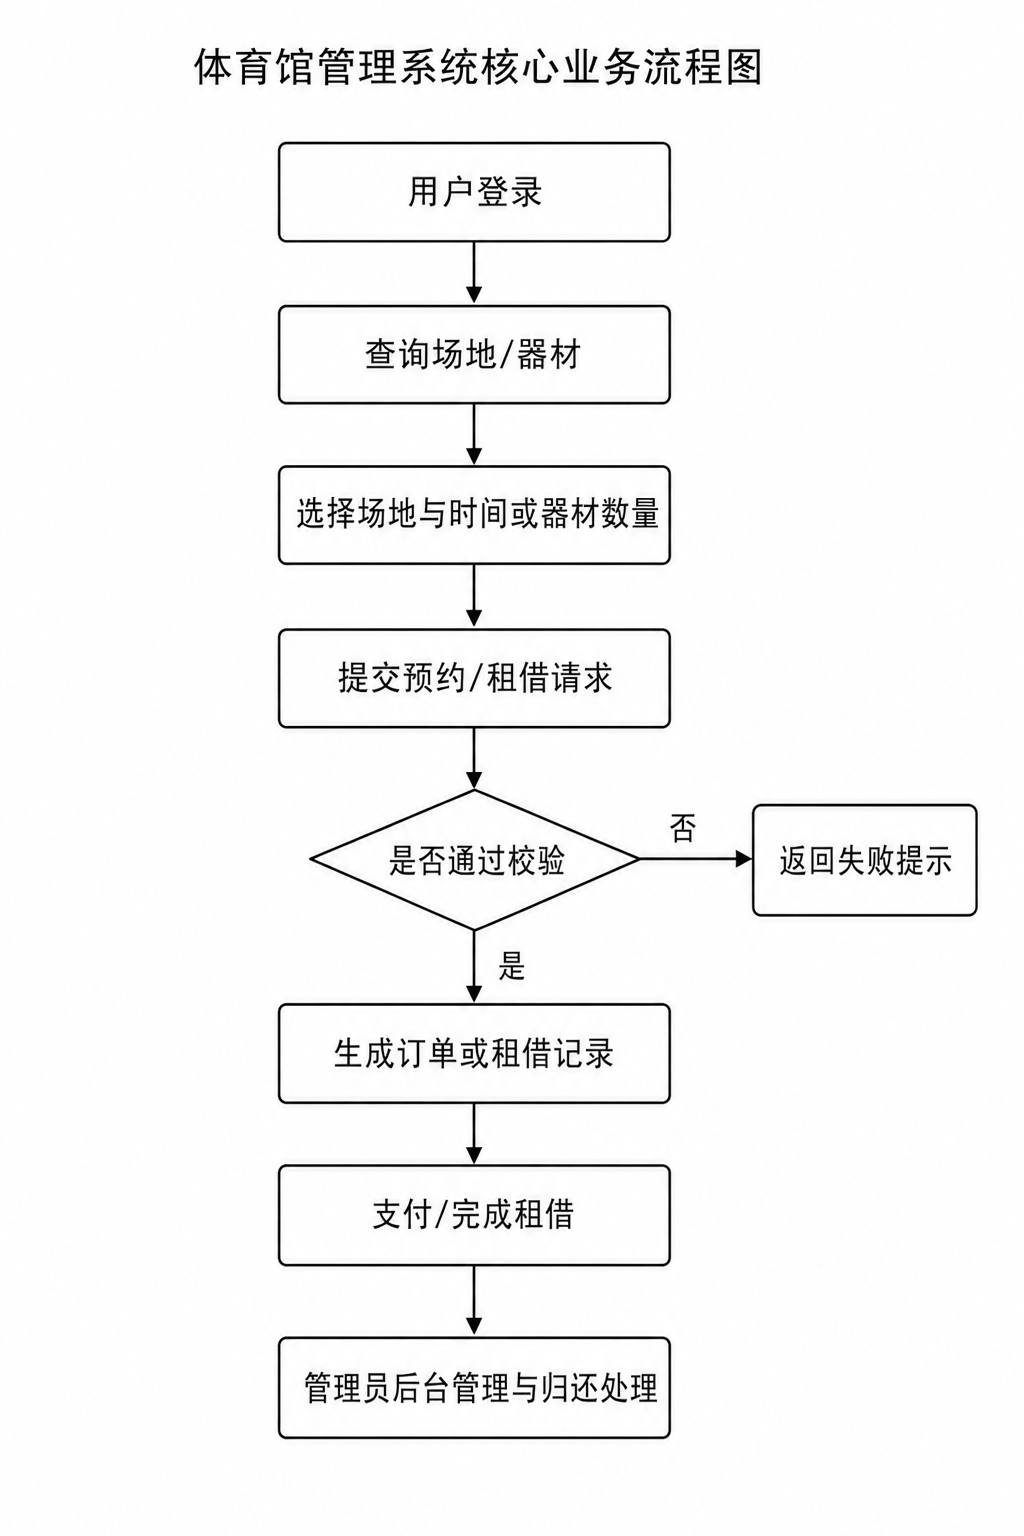
\includegraphics[width=0.82\textwidth]{img/fig4-3.png}
\caption{核心业务流程图}
\label{fig:process-placeholder}
\end{figure}

\section{数据库设计}

\subsection{数据库概念结构设计}

概念结构这一步主要是从业务里抽象出"东西"。本系统抽出了六个核心实体：角色、用户、场地、订单、器材、租借记录。它们之间的关系并不复杂——一个角色对应多个用户，一个用户可以下多个订单，一个场地也可以承载多个订单；器材和租借记录之间通过租借数量、归还状态来反映库存的变化。这些关系合在一起，就构成了系统的业务语义\cite{wan2016}。把它们画成 ER 图，能比较直观地看到各个对象的位置和走向，也方便后面落到具体的数据表上。

\begin{figure}[htbp]
\centering
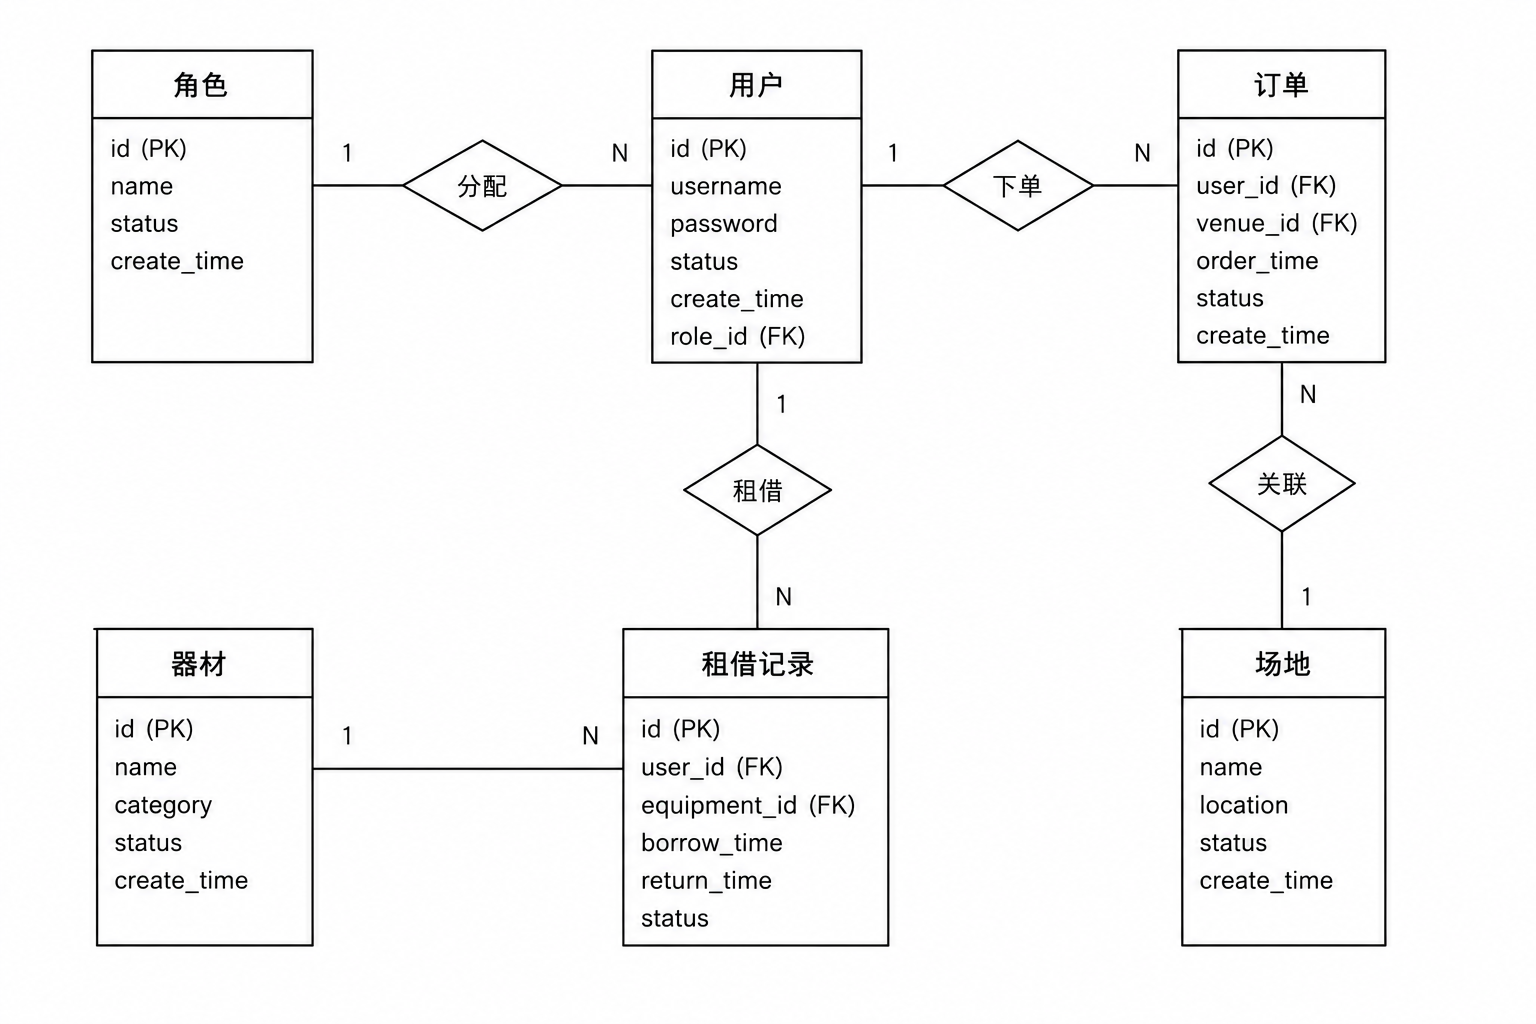
\includegraphics[width=0.82\textwidth]{img/fig4-4.png}
\caption{数据库 ER 图}
\label{fig:er-placeholder}
\end{figure}

\subsection{数据库逻辑结构设计}

下一步把概念模型落到 MySQL 的具体表上，给每张表定字段、主键、外键和必要的约束。结合项目里的初始化脚本，系统一共有六张业务表：角色表、用户表、场地表、订单表、器材表、租借记录表。它们各自负责一类数据，外键和状态字段把彼此连起来——例如订单表里同时持有 user\_id 和 venue\_id，租借记录表持有 user\_id 和 equipment\_id。下面几张表给出每张表的字段细节。

\begin{table}[htbp]
\centering
\caption{角色表结构设计}
\label{tab:role-table}
\small
\begin{tabularx}{\textwidth}{p{2.2cm}p{2.7cm}p{2.4cm}X}
\toprule
字段名 & 数据类型 & 约束 & 字段说明 \\
\midrule
id & BIGINT & 主键，自增 & 角色编号 \\
name & VARCHAR(50) & 非空，唯一 & 角色名称，取值为 admin 或 user \\
\bottomrule
\end{tabularx}
\end{table}

\begin{table}[htbp]
\centering
\caption{用户表结构设计}
\label{tab:user-table}
\small
\begin{tabularx}{\textwidth}{p{2.2cm}p{2.7cm}p{2.4cm}X}
\toprule
字段名 & 数据类型 & 约束 & 字段说明 \\
\midrule
id & BIGINT & 主键，自增 & 用户编号 \\
username & VARCHAR(50) & 非空，唯一 & 用户名 \\
password & VARCHAR(100) & 非空 & 登录密码 \\
phone & VARCHAR(20) & 可空 & 用户手机号 \\
role\_id & BIGINT & 非空，外键 & 对应角色编号 \\
create\_time & DATETIME & 非空 & 用户创建时间 \\
\bottomrule
\end{tabularx}
\end{table}

\begin{table}[htbp]
\centering
\caption{场地表结构设计}
\label{tab:venue-table}
\small
\begin{tabularx}{\textwidth}{p{2.2cm}p{2.7cm}p{2.4cm}X}
\toprule
字段名 & 数据类型 & 约束 & 字段说明 \\
\midrule
id & BIGINT & 主键，自增 & 场地编号 \\
name & VARCHAR(100) & 非空 & 场地名称 \\
type & VARCHAR(50) & 非空 & 场地类型 \\
status & TINYINT & 非空，默认 1 & 场地状态 \\
open\_time & TIME & 非空 & 开放开始时间 \\
close\_time & TIME & 非空 & 开放结束时间 \\
\makecell[l]{price\_per\_\\hour} & DECIMAL(10,2) & 非空 & 每小时价格 \\
create\_time & DATETIME & 非空 & 创建时间 \\
\bottomrule
\end{tabularx}
\end{table}

\begin{table}[htbp]
\centering
\caption{订单表结构设计}
\label{tab:order-table}
\small
\begin{tabularx}{\textwidth}{p{2.2cm}p{2.7cm}p{2.4cm}X}
\toprule
字段名 & 数据类型 & 约束 & 字段说明 \\
\midrule
id & BIGINT & 主键，自增 & 订单编号 \\
order\_no & VARCHAR(32) & 非空，唯一 & 订单号 \\
user\_id & BIGINT & 非空，外键 & 下单用户编号 \\
venue\_id & BIGINT & 非空，外键 & 预约场地编号 \\
book\_date & DATE & 非空 & 预约日期 \\
start\_time & TIME & 非空 & 开始时段 \\
end\_time & TIME & 非空 & 结束时段 \\
total\_amount & DECIMAL(10,2) & 非空 & 订单总金额 \\
status & TINYINT & 非空，默认 0 & 订单状态 \\
create\_time & DATETIME & 非空 & 订单创建时间 \\
\bottomrule
\end{tabularx}
\end{table}

\begin{table}[htbp]
\centering
\caption{器材表结构设计}
\label{tab:equipment-table}
\small
\begin{tabularx}{\textwidth}{p{2.2cm}p{2.7cm}p{2.4cm}X}
\toprule
字段名 & 数据类型 & 约束 & 字段说明 \\
\midrule
id & BIGINT & 主键，自增 & 器材编号 \\
name & VARCHAR(100) & 非空 & 器材名称 \\
total\_qty & INT & 非空 & 器材总数量 \\
available\_qty & INT & 非空 & 当前可借数量 \\
\makecell[l]{price\_per\_\\hour} & DECIMAL(10,2) & 非空 & 每小时租借价格 \\
create\_time & DATETIME & 非空 & 创建时间 \\
\bottomrule
\end{tabularx}

\vspace{1.5em} % 两表之间的间距

\caption{租借记录表结构设计}
\label{tab:rental-table}
\small
\begin{tabularx}{\textwidth}{p{2.2cm}p{2.7cm}p{2.4cm}X}
\toprule
字段名 & 数据类型 & 约束 & 字段说明 \\
\midrule
id & BIGINT & 主键，自增 & 租借记录编号 \\
user\_id & BIGINT & 非空，外键 & 租借用户编号 \\
equipment\_id & BIGINT & 非空，外键 & 器材编号 \\
quantity & INT & 非空 & 租借数量 \\
status & TINYINT & 非空，默认 0 & 租借状态 \\
create\_time & DATETIME & 非空 & 租借时间 \\
return\_time & DATETIME & 可空 & 归还时间 \\
\bottomrule
\end{tabularx}
\end{table}
